%%This is a very basic article template.
%%There is just one section and two subsections.
\documentclass[a4paper,12pt]{article}
\usepackage{my-main}
\newfloat{algo}{thp}{lop}
\floatname{algo}{Алгоритм}
\bibliographystyle{plain}

\begin{document}
\begin {titlepage}
  \newpage
  \begin {center}
    Московский государственный университет имени  М. В. Ломоносова\\
    Факультет вычислительной математики и кибернетики\\
    Кафедра системного программирования \\
  \end {center}
  \vspace {5cm}
  \begin {center}
    \LARGE {Курсовая работа}\\
    \Large {Организация вычислений на системе с ускорителем}
  \end {center}
  \vspace {1cm}
  \begin {flushright}
    Выполнил:\\
    студент 427 группы\\
    Платонов В.\,А.\blb
    Научный руководитель:\\
    доцент, к.ф.-м.н. Гайсарян С.\,С.
  \end {flushright}
  \vspace{\fill}
  \begin {center}
  Москва, 2011
  \end {center}
\end {titlepage}

\tableofcontents
\newpage

\section{Постановка задачи}
Основным вычислительным устройством в большинстве современных компьютеров
является процессор общего назначения. Он обладает некоторым
заранее определённым набором команд, на которые и разбивается любая задача.
Основным способом увеличения производительности подобных устройств является
повышение количества выполнений данных операций в единицу времени. Для
вычислительно ёмких задач используются системы из таких процессоров и коммуникации между ними. 
Другим способом ускорения вычислений является создание специализированных
процессоров для конкретной задачи. Аппаратная реализация позволяет получить существенный выигрыш
производительности, однако практическая стоимость подобных устройств очень
велика и они ограничены решением только одной задачи. В связи с этим сначала
возникла, а потом реализовалась идея программируемых логических устройств,
которые позволяют пользователю с помощью некоторого языка описания настроить
устройство для решения конкретной задачи. Хотя вычислительная мощность подобных плат и уступает
чисто аппаратной реализации, возможность
перепрограммирования, скорость разработки и ввода в производство, а также
стоимость делают их очень привлекательными. Решение какой - то конкретной
проблемы может как целиком быть перенесено на такое устройство(или систему из
них), так и выполняться на обычном процессоре, с использованием устройства в
качестве ускорителя для некоторых частей программы.
\section{Обзор предметной области}
\subsection{FPGA}
\subsubsection{Общая информация}

FPGA состоит из:
\begin{itemize}
  \item Логических блоков, реализующих базовые операции
  \item Блоков ввода-вывода
  \item Внутренних связей
\end{itemize}

Логические блоки имеют некоторое количество входов и выходов, реализуя
произвольную логическую функцию от соответствующего числа аргументов на любом
своем выходе.

Блоки ввода-вывода обеспечивают связь между контактами корпуса и внутренними
связями.

Внутренние связи организованы в виде вертикальных и горизонтальных каналов,
состоящих из нескольких связей. На пересечении каналов находятся блоки
переключения, позволяющие подключать связи из канала, входящего в блок к
соответствующим связям из оставшихся трех каналов. Схема блока переключения,
находящегося на пересечении четырех связей, показана на рисунке \ref{fpga-cell}.

\begin{figure}
\includegraphics [width=\textwidth]{pictures/cell}
\caption{Схема блока переключения FPGA}
\label{fpga-cell}
\end{figure}

\subsubsection{Задачи, решаемые на FPGA}

В данное время, основные производители FPGA устройств такие как Xilinx и Altera
предлагают свои решения для различных областей рынка, таких как:

\begin{enumerate}
	\item Аэрокосмическая
	\item Оборонная
	\item Автомобильная
	\item Сфера обслуживания
	\item Высокопроизводительные вычисления
	\item Хранение данных
	\item Проводные и беспроводные соединения
	\item Автоматизация индустриальных процессов
	\item Медицинская
	\item Телекоммуникационная
\end{enumerate}

Фактически, все эти решения предполагаю использования FPGA в одном из следующих
вариантов:

\begin{enumerate}
  \item Независимое вычислительное устройство(stand - alone)
  		\begin{enumerate}
  		  \item Цифровая обработка сигналов(DSP)
  		  		Долгое время FPGA не могли сравниться в производительности с DSP
  		  		процессорами, но постепенное развитие: увеличение числа логических
  		  		блоков, появления специализированных DSP блоков, добавление
  		  		мультиплексоров, повышение тактовой частоты, позволили стать
  		  		конкурентноспособными. Кроме того, на определённых задачах, возможности
  		  		параллельной обработки, дают резкий прирост производительности.

  		  \item Реализация логики управления некоторым устройством.
  		  		Электронные устройства или некоторая система из них нуждается в
  		  		непосредственном управлении. Разумеется, можно использовать для этого
  		  		ASIC устройства, однако цена такого решения высока. Потому огромной
  		  		популярностью пользуются реализации на FPGA устройствах. 
  		  		Наиболее широко используются такие решения в силовая
  		  		электронике. К примеру, в самолёте Airbus 380 находится
  		  		по меньшей мере 700 FPGA чипов. Согласно проведённым исследованиям,
  				добавление логики управления на FPGA чипе для всех электромоторов в США,
  				позволит экономить в год 15 млрд. \$.
  		\end{enumerate}
  \item Акселератор
  		Аппаратная реализация алгоритма, широкие возможности для параллельного
  		исполнения, экономное энергопотребление делают устройство привлекательным
  		для выполнения как научных так и прикладных вычислений. Существуют уже
  		готовые вычислительные системы состоящие как из обычных центральных
  		процессоров так и блоков FPGA акселераторов Примерами прикладных задач
  		являются: декодирование видео и аудио потоков, криптографические задачи,
  		ускорение работы баз данных, обработка финансовых данных.
  \item Прототипирование
    	FPGA являются основой текущей мейнстримовой методологии аппаратной
  		верификации ASIC и SoC а также раннего проектирования проектирования
  		программного обеспечения и прошивок. Компания Intel проектировала на системе
  		FPGA кристаллов процессоры Intel Atom и Intel Nehalem. 
\end{enumerate}


\subsection{OpenCL}
OpenCL  — фреймворк для 
написания параллельных программ для различных платформ, включающих в
себя центральные процессоры и графические ускорители . В фреймворк OpenCL входят
язык программирования для акселератора, который базируется на стандарте C99, и
интерфейс для программы выполняющихся на центральном процессоре. OpenCL является
полностью открытым стандартом, разрабатывается и поддерживается некоммерческим консорциумом Khronos Group, 
в который входят много крупных компаний, включая Apple, AMD, Intel, nVidia, Sun Microsystems, Sony 
Computer Entertainment и другие.

Программная модель OpenCL позволяет программисту описывать функции, которые будут
параллельно выполнены на некотором акселераторе или наборе акселераторов, доступных на
данной машине.
В основе программной модели OpenCL лежит понятия ядра (kernel). Ядро — это функция,
которая будет выполнена параллельно на акселераторе определенным количеством
потоков. Ядра создаются, компилируются и запускаются программой на хосте, с помощью
вызовов функций библиотеки OpenCL. Запуск нужного ядра с указанием требуемого количества потоков
осуществляется с помощью вызова функции библиотеки OpenCL на центральном
процессоре. Таким образом, программа состоит из последовательного кода, который выполняется
на центральном процессоре и параллельного кода, которые выполняется на
акселераторе.

\section{OpenCL для FPGA}
FPGA-OpenCL - система автоматизации вычислений на FPGA-ускорителях на основе
 стандарта OpenCL. В неё входят следующие компоненты:
\begin{enumerate}
   \item Реализация некоторого подмножества OpenCL достаточного для работы с
   FPGA.
   \item Механизм обмена данными.
   \item Диспетчер запросов на выполнение команд на акселераторе.
   \item Драйвер для осуществления взаимодействия между устройством и
   центральным процессором.
   \item Генерация прошивки для устройства на основе созданных OpenCL ядер.
\end{enumerate}

Общая схема работы FPGA-OpenCL:

\begin{figure}[h!]
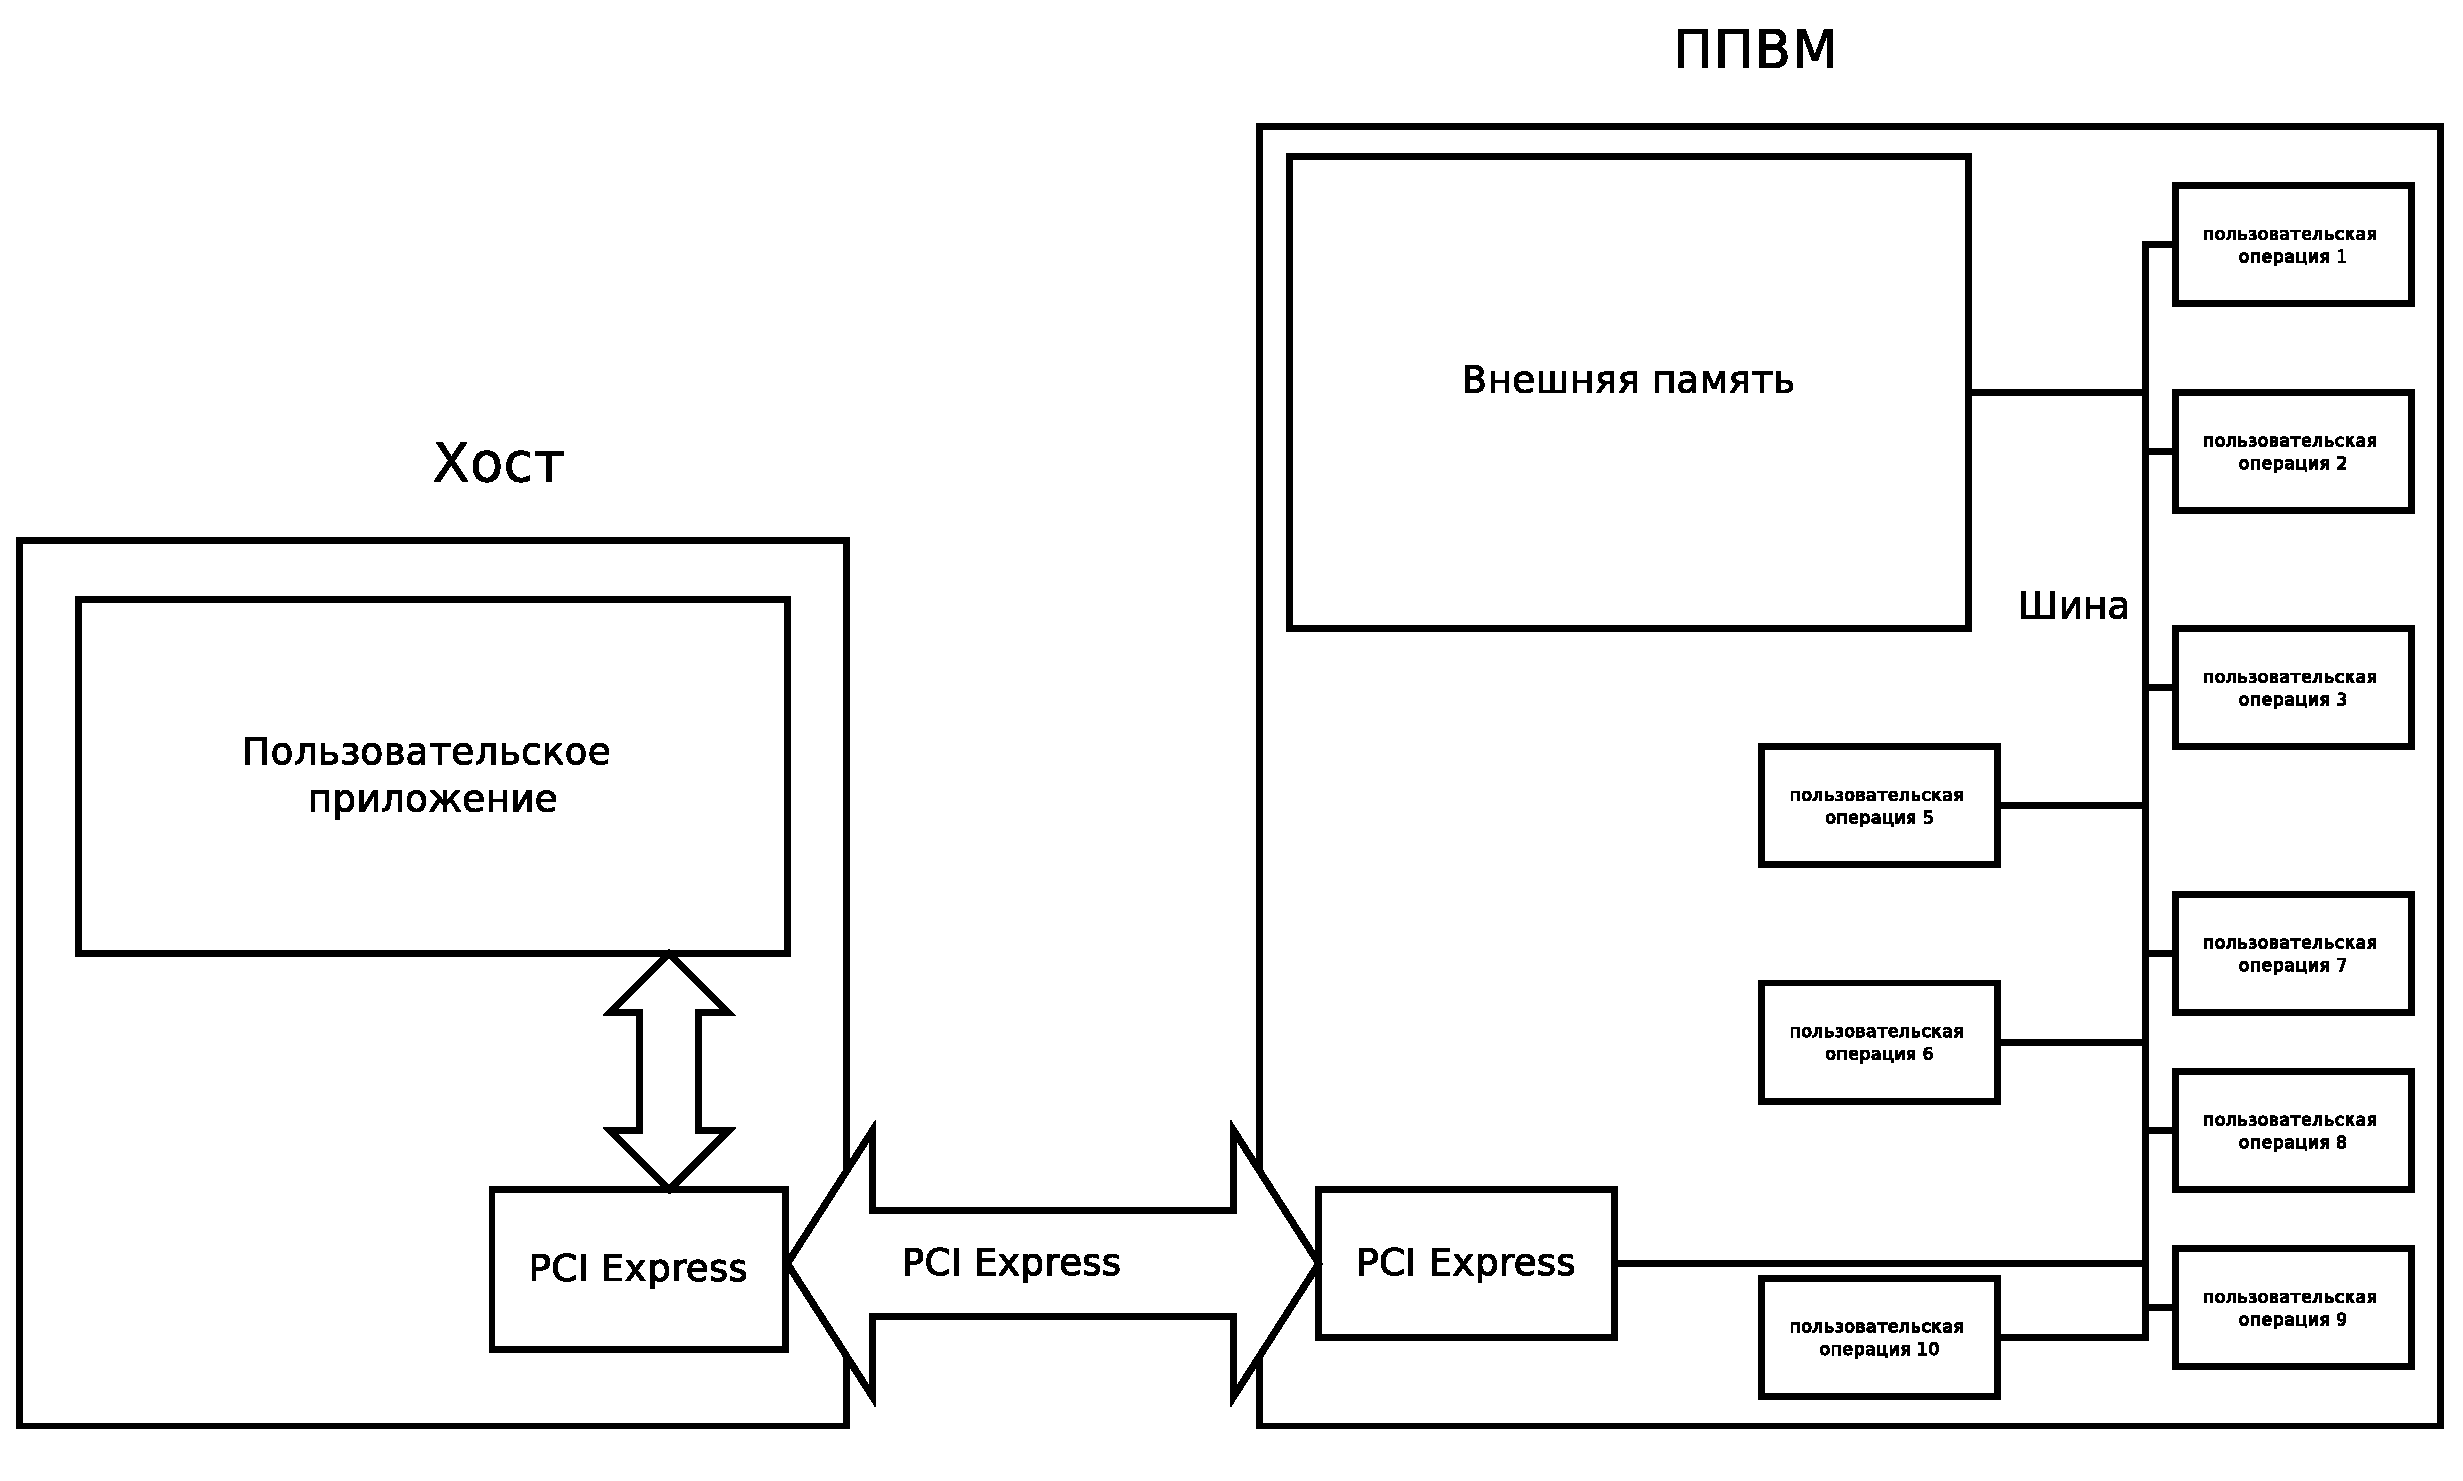
\includegraphics [width=\textwidth]{pictures/base-scheme}
\caption{Общая схема работы FPGA-OpenCL}
\label{fpga-cell}
\end{figure}

В рамках данной работы были произведены две реализации диспетчера задач. Первая
реализация работала на софтверном процессоре акселератора, вторая была размещена
непосредственно в драйвере.
\section{Диспетчер задач}
\subsection{Реализация на microblaze}
Диспетчер представляет собой некоторую программу, работающую на процессоре
Microblaze, расположенном на FPGA плате. 
В обязанности диспетчера входят следующие вещи:
\begin{enumerate}
  \item Приём новых задач для выполнения от хоста.
  \item Распределение задач в соответствие с имеющимися ресурсами.
  \item Отслеживание завершения работы задачи и информирование хоста об этом.
\end{enumerate}

Так как Microblaze является программным процессором, диспетчер должен быть,
по возможности, простым и не требующим больших ресурсов.
Для общения с хостом, используется BRAM память, подключённая к Microblaze через
PLB шину. Она невелика по размерам(и разбита на страницы по 4 килобайта),
двухпортовая и синхронная. Одна такая страница отображена в BAR0 PCIe Core,
и через неё происходит обмен сообщениями. Остальная память используется
диспетчер.

В отображённой области памяти статически выделены смещения, по которым будет
происходить запись.
\begin{enumerate}
  \item 0x4 - флаг \texttt {HOST\_DONE}
  \item 0x8 - флаг \texttt {FPGA\_DONE}
  \item 0x14 - адрес для записи результата обработки команды
  \item 0x18 - адрес для записи размера команды
  \item 0х44 - адрес с которого начинается записанная команда.
\end{enumerate}

Для синхронности обмена сообщениями используется следующий протокол, он
представлен на рисунке \ref{mb-sch-auto}. Есть два флага \texttt {HOST\_DONE} и
\texttt {FPGA\_DONE}. Поднятый первый флаг означает, что хост записал своё
сообщение и диспетчер может его обрабатывать. Поднятый второй флаг означает, что
запрос был успешно обработан. Начальное состояние флагов (0,1) задаётся
диспетчером при запуске.
\begin{enumerate}
  \item Состояние флагов (0,1). Хост опускает второй флаг и начинает запись
  сообщения и/или анализ возвращённого значения. По окончании флаги
  устанавливаются в (1, 0)
  \item Состояние флагов (1,0). Диспетчер начинает обработку команды, по
  окончании он записывает результат операции и переводит флаги в (0,1).
\end{enumerate}

\begin{figure}
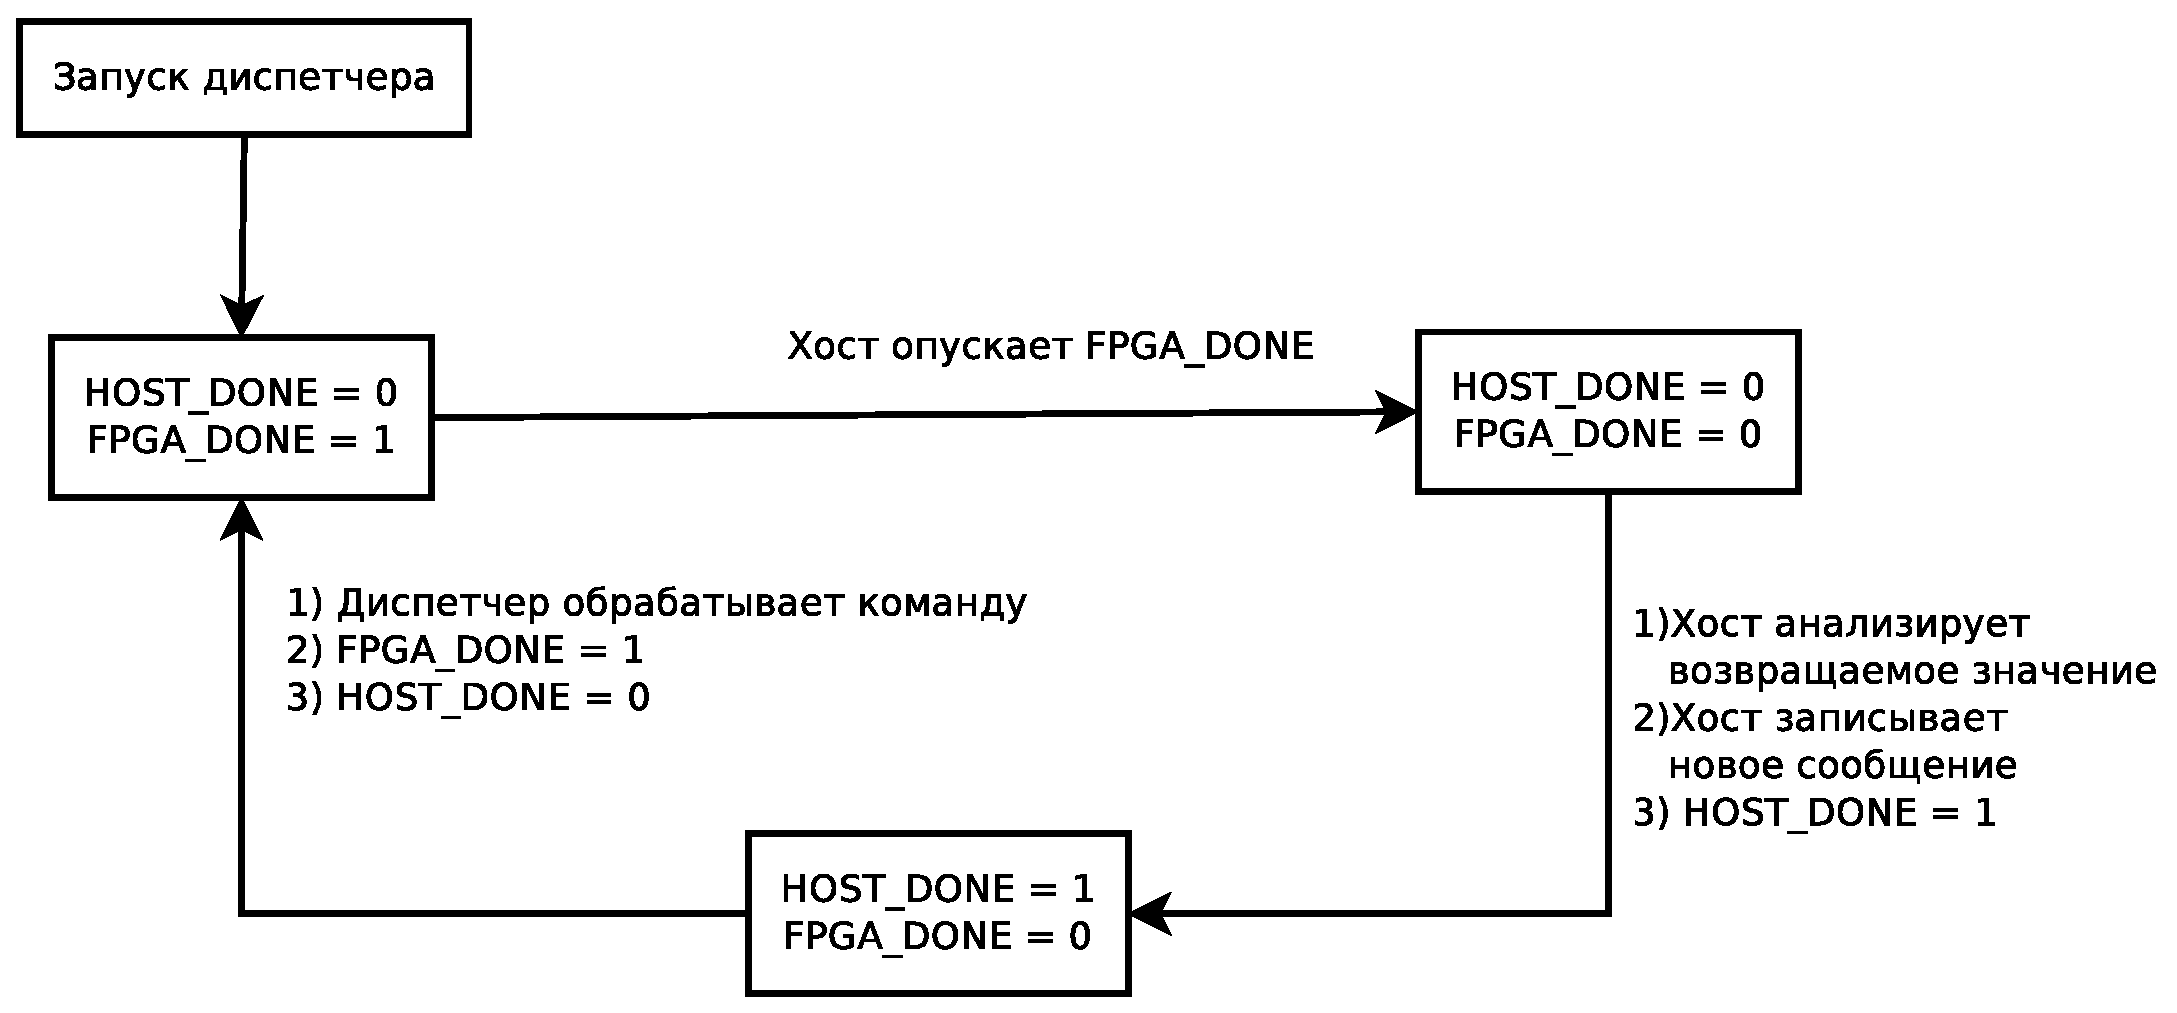
\includegraphics [width=\textwidth]{pictures/mb_sch_auto}
\caption{Протокол обмена сообщениями}
\label{mb-sch-auto}
\end{figure}

Команда имеет следующий формат:\\
<\texttt {kernel\_id} (4 bytes)><\texttt {job\_id} (8 bytes) > \{\texttt{args}\} ~\\

Здесь \texttt {kernel\_id} - уникальный номер ядра, на котором должна
обрабатываться задача, \texttt{job\_id} - уникальный номер задания,
\texttt{args} - аргументы для запуска задачи.

Каждое ядро в системе описывается структурой, хранящей в себе его уникальный
номер, статус(было ли ядру дано какое-либо задание), функция, осуществляющая
запуск задания на нём и функция осуществляющая проверку того, что ядро
закончило работу(например чтение каких-то регистров результата). При
поступление нового задания, обработчик сначала создаёт структуру-обёртку, в
которую, в частности, сохраняются аргументы запуска. Затем в списке ядер ищется
соответствующее заданию ядро и, если оно свободно, задание сразу же
запускается. В противном случае, оно добавляется в очередь заданий для данного
ядра. Таким образом, для добавления в диспетчер поддержки нового ядра,
необходимо написать два обработчика(запуска и проверки результата) и добавить с
структуры данных диспетчера информацию об этом ядре.

В диспетчере постоянно производится опрос ядер на факт завершения выполнения
на них какого-либо задания. Для этого у каждого из имеющихся ядер сначала
проверяется его статус, а затем, если ядру было дано какое-то задание, то
проверяется статус его выполнения. Если какое-то задание завершилось,
в специальный регистр записывается номер задания, а устройство посылает
прерывание, фиксируемое драйвером.  После того, как мы убедимся, что хост считал
номер выполненного задания, при наличии в очереди следующей задачи для этого
ядра, она запускается на нем.

Таким образом всю работу диспетчера можно представить в следующем виде.

  \begin{algo}
\begin{algorithmic}
	\STATE $scheduler\_initialization()$
	\STATE $BRAM\_initialization()$
	\WHILE {\TRUE}
		\STATE $check\_kernels()$
		\IF {$have\_new\_message()$}
			\STATE $process\_message()$
			\STATE $set\_flags()$
		\ENDIF
	\ENDWHILE
\end{algorithmic}
  \caption{Алгоритм работы планировщика}
  \end{algo}
  
Данная реализация справлялась с поставленными задачами, однако по некоторому
размышлению, была предложена новая концепция диспетчера, которая позволяла
перенести его из microblaze в драйвер ядра. Это позволит убрать требование
наличия в целом софтверного процессора на устройстве и избежать активного
ожидания при опросе ядер.

\subsection{Реализация в модуле ядра}
Планировщик расположен в драйвере для
устройства и работает соответственно на центральном прцоессоре.
Непосредственное общение с устройством сократилось до запуска задач, с помощью
записи некоторых значений по определённым адресам. В остальном, драйвер по
необходимости вызывает функции планировщика и скрывает от него общение с
устройством. В обязанности планировщика входят следующие вещи:
\begin{enumerate}
  \item Приём новых вычислительных задач для выполнения,их сериализация и
  запуск.
  \item Приём новых задач DMA-транзакций, их сериализация и запуск
  \item Информирование драйвера о проблемах при запуске задачи.
  \item Обеспечение корректности выдачи уникальных идентификаторов ядрам.
\end{enumerate}

Экземпляр планировщика создаётся при загрузке модуля драйвера. При добавлении в
систему устройства, для него создаётся соответствующая структура. Далее драйвер
должен задать планировщику сколько и какие ядра будут на устройстве, планировщик
сам назначит им набор уникальных, подряд идущих номеров и вернёт первое значение
драйверу. Теперь возможны запуски задач. У каждого ядра есть своя очередь задач,
на выполнение. Кроме того есть отдельная очередь под
DMA-транзакции.  Планировщик только выполняет запуск задач. Драйвер сам
отслеживает окончание работы и сообщает об этом планировщику, чтобы тот запустил
следующую задачу(если таковая имеется). В случае возникновения ошибки при
запуске, планировщик сообщает об этом драйверу и пытается запустить следующую
задачу. При удалении устройства, удаляется соответствующая структура, все ядра и
очереди задач на них. В процессе работы возможно переустановление ядер для
устройства, в этом случае старые ядра и очереди задач на них удаляются. 

\section{Результаты}
Реализованная в рамках данной работы система удовлетворяет исходной постановке
задачи, предоставляя программисту стандартный набор операций для работы с ППВМ
как OpenCL акселераторами. Полученная система тестировалась на ППВМ Xilinx
Virtex-6 (XC6VLX240T)\cite{virtex-6-overview}.

Числовые характеристики работы системы приведены в таблице \ref{results-table}.
\begin{table}[h!]
\caption{Характеристики работы системы}
\begin{center}
\begin{tabular}{|c|c|}
\hline
Скорость записи в память устройства & $986.2$ Мб/сек \\ \hline
Скорость чтения из памяти устройства & $1246.9$ Мб/сек \\ \hline
Задержка запуска ядра & $\sim 7-8$ мкс \\ \hline
Задержка ожидания некоторого события & $\sim 8-10$ мкс \\ \hline
Время запуска ядра & $\sim 100-150$ мкс \\ \hline
Задержка запуска обмена данными & $\sim 8-10$ мкс. \\ \hline
Время перепрограммирования устройства & $\sim 25$ сек \\\hline
\end{tabular}
\end{center}
\label{results-table}
\end{table}

При этом, необходимо отличать задержку запуская ядра (время, прошедшее между
вызовом \texttt{clEnqueueNDRangeKernel} и возвратом из нее) и время запуская
ядра, включающее в себя время выполнения всех необходимых операций в
параллельном потоке очереди команд.
\section{Заключение}
В рамках данной работы была проведена разработка планировщика заданий системы
автоматизации программирования для FPGA. Были предложены две реализации, одна
размещала планировщик на софтверном процессоре устройства, другая располагала
его в драйвере устройства. Текущая версия поддерживает несколько устройств с
уникальным набором ядер, очередей задач для них и DMA-очередей. 

В рамках
планировщика в будущем планируется использовать механизм частичной реконфигурации ППВМ для
замены ядер, работающих на FPGA без полного перепрограммирования FPGA
\cite{partial-reconfiguration-report}. Кроме того, планируется реализации
конвееризации для имеющихся ядер с перенаправлением вывода одного ядра на вход
другого, с целью извлечения дополнительного параллелизма.


\newpage
\addcontentsline {toc}{section}{\text{Список литературы}}
\bibliography{biblio/ref}
\end{document}
